\chapter{Discussion and Conclusions}
\label{chap:conclusions}
\label{chap:discussion}

\section{The Central Finding: AUROC Misranks Models for the Clinical OOD Task}
\label{sec:central_finding}

The argument is organized around a single empirical observation that contradicts what the field assumes: the metric used to rank models on internal leaderboards, the area under the receiver operating characteristic curve (AUROC), does not predict which model is useful for the real clinical task, namely detecting disease in an out-of-distribution (OOD) patient population. This observation leads to three further developments: a taxonomy that separates two qualitatively different OOD failure modes, an OOD-sensitivity ranking that turns out to invert the AUROC ranking, and a comparison between physics-based and phenomenological inductive biases. Throughout, the inviolable rule established in Chapter~\ref{chap:research} is observed: metrics belonging to different evaluation groups (A, B, and C) are never compared as if they were commensurable.

The defining result of this thesis is a contrast between two Group-C models evaluated on the same held-out CODE-15\% set and the same isolated SaMi-Trop OOD cohort.

Approach~12, the fine-tuned DeepECG-SSL model, attains the highest CODE-15\% held-out AUROC of any approach in the thesis: $0.8593$ (95\% CI $[0.8484,\,0.8716]$). On the conventional leaderboard it is unambiguously the best discriminator. Yet when this same model is applied at its default decision threshold to the SaMi-Trop cohort, a population it never saw during training, it identifies none of the positive patients: its OOD sensitivity is exactly $0.0000$. Because the SaMi-Trop test set contains a single class, AUROC is undefined there, so the in-distribution figure of merit cannot even be computed on the population that matters.

Approach~11, the McSharry autoencoder, presents the mirror image. It has the \emph{lowest} CODE-15\% AUROC in Group~C, $0.7710$ (95\% CI $[0.7555,\,0.7873]$). By the leaderboard it is the weakest of the four Group-C models. On the SaMi-Trop cohort, however, the disease signal is plainly present: the mean predicted OOD score is $0.3331$, and a single adjustment of the decision threshold from the default $0.5$ to $0.1$ recovers $99.45\%$ of the cohort (sensitivity $0.9945$, $1622/1631$).

\begin{figure}[htbp]
    \centering
    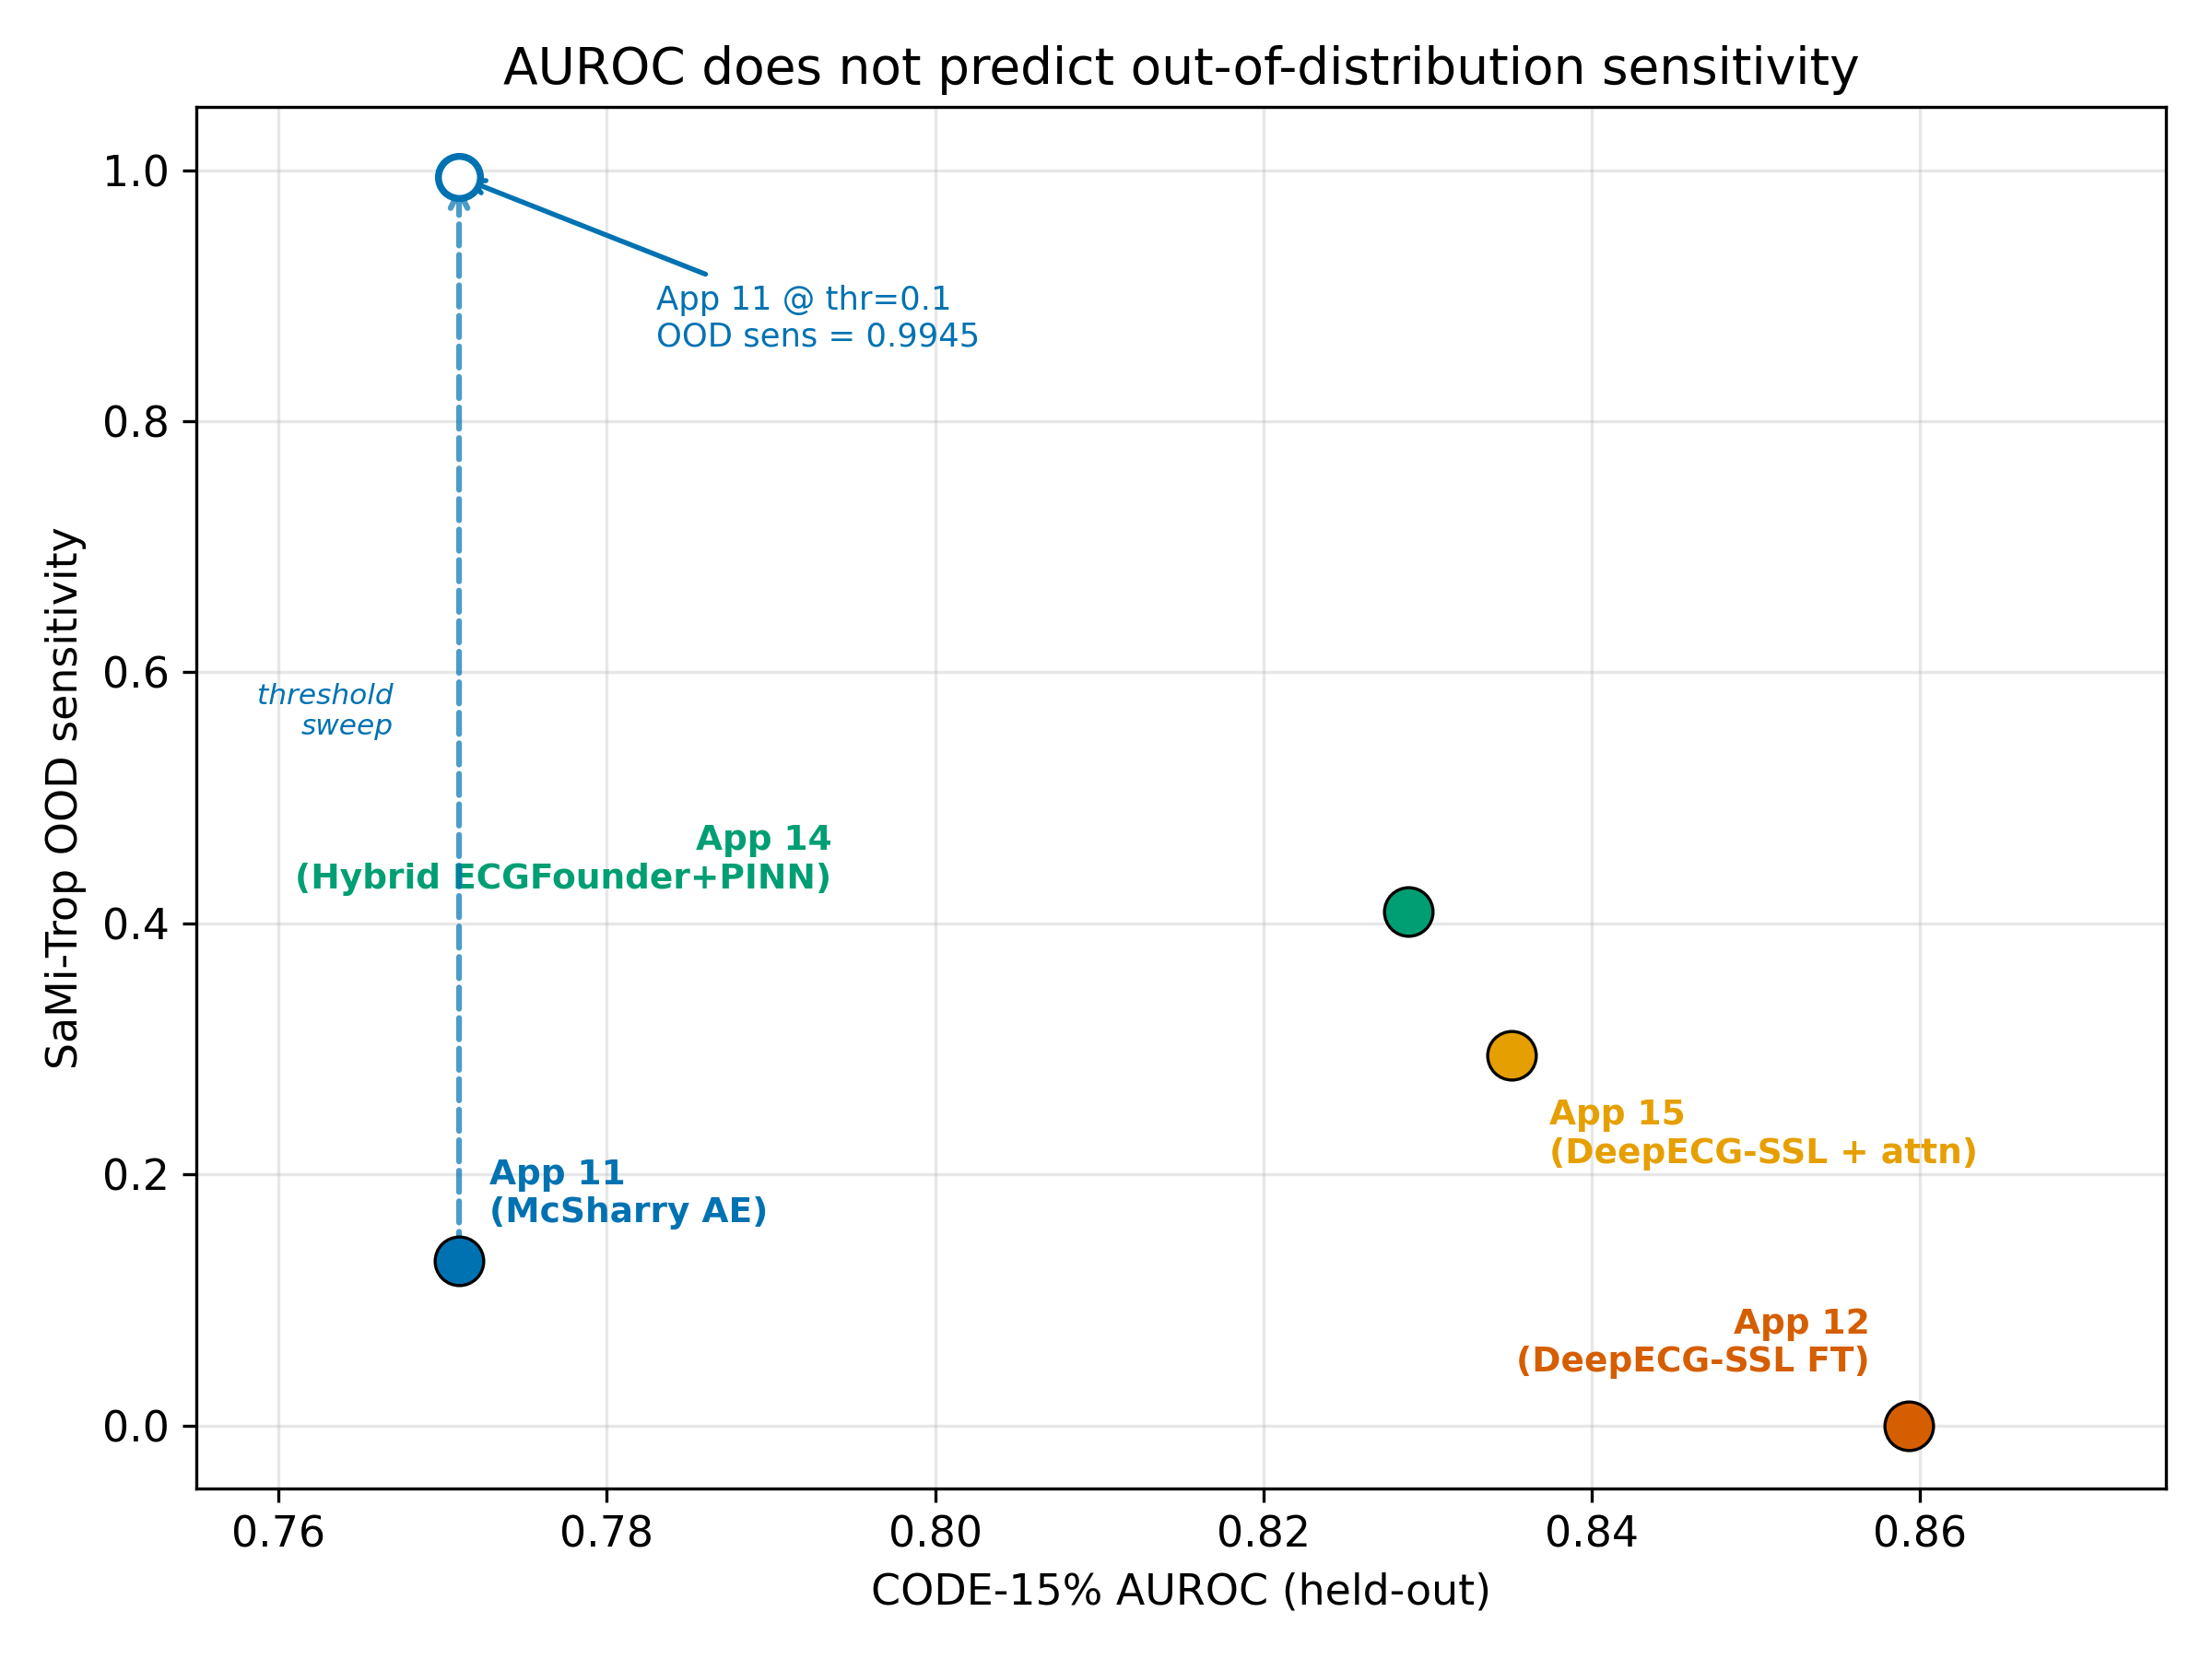
\includegraphics[width=0.85\linewidth]{img/auroc_vs_ood}
    \caption[OOD sensitivity vs.\ in-distribution AUROC for Group-C approaches]{Out-of-distribution sensitivity on the SaMi-Trop cohort as a
    function of in-distribution AUROC on CODE-15\% for the four Group-C
    approaches. A high AUROC does not translate into out-of-distribution
    sensitivity: Approach~12 attains the highest AUROC yet zero OOD sensitivity
    at its default threshold, whereas Approach~11 detects $99.45\%$ of the cohort
    once its threshold is lowered to $0.1$ (dashed arrow). Selecting a model by
    AUROC alone would deploy the worst performer for the clinical screening task.}
    \label{fig:auroc_vs_ood}
\end{figure}

Placed side by side (Figure~\ref{fig:auroc_vs_ood}), these two facts establish the central claim. A threshold-independent, in-distribution discriminative metric does not predict OOD screening sensitivity. It also ranks the two models in the wrong order for the clinical task: the model that the AUROC leaderboard crowns (Approach~12) is the one that, deployed as-is, would miss every Chagas-positive patient in the endemic cohort, whereas the model the leaderboard relegates to last place (Approach~11) is the one whose latent signal can be turned into near-complete OOD recall with a single threshold move. A practitioner who selected a model by AUROC alone would deploy the wrong system. This is the answer to RQ5, posed in Chapter~\ref{chap:introduction}: threshold-independent discriminative performance does \emph{not} rank models correctly for the real clinical out-of-distribution screening task.

The deeper reason is that AUROC rewards the \emph{separability} of scores within a fixed distribution while saying nothing about where those scores land relative to a deployed threshold once the distribution shifts. A model can rank in-distribution positives above in-distribution negatives very well (high AUROC) and still map an entire shifted population below its operating point (zero sensitivity at the default cutoff). For a screening instrument, whose entire value lies in catching cases under distribution shift, this is the failure that matters, and it is exactly the one AUROC is blind to.

\section{Two Distinct Out-of-Distribution Failure Modes}
\label{sec:failure_modes}

It would be a mistake to lump every OOD shortfall together. The results expose two qualitatively different failure modes, and conflating them would obscure the only one that admits a cheap remedy.

The first mode is a genuine \emph{Clever Hans} failure, and the term is reserved here for Approach~10, the McSharry phenomenological PINN, alone. Approach~10 achieves a strong in-distribution validation AUROC of $0.8273$ on CODE-15\% yet, the hypothesis holds, carries no transferable disease signal to a shifted population. This is a hypothesis, not a measured number: the committed notebook of record for Approach~10 contains no test-evaluation cell, so no SaMi-Trop sensitivity was actually recorded, and none is asserted here. The hypothesis is grounded instead in two structural facts. First, the model's parametrization is richly over-specified for the task: it exposes seventeen free phenomenological parameters, including a baseline-offset term $z_0$ that captures the recording's isoelectric line, an equipment- and acquisition-specific artifact rather than a marker of cardiac pathology~\cite{mcsharry2003dynamical}. A model with that many degrees of freedom can fit the validation distribution by leaning on such artifacts, in the manner of Clever Hans answering not the question asked but a spurious cue correlated with it~\cite{muller2019does}. Second, the OOD test set is single-class, which means a Clever-Hans model anchored to source-domain artifacts would have no opportunity to be corrected and every opportunity to fail silently. The claim about Approach~10 is therefore architectural and evidential, not a quantitative measurement.

The second mode is entirely different and is exemplified by Approach~11: a \emph{calibration} or \emph{threshold-shift} failure. Here the transferable disease signal is demonstrably present. The mean predicted OOD score on SaMi-Trop is $0.3331$, well above zero and concentrated in a region the model treats as mildly suspicious. The failure is not that the model cannot see the disease; it is that the default $0.5$ decision threshold sits above where the OOD scores accumulate, suppressing a signal the model has in fact extracted. Lowering the threshold to $0.1$ converts that latent signal into $99.45\%$ sensitivity. This is a miscalibration of the operating point under distribution shift, the kind of problem that post-hoc threshold or probability recalibration is designed to address~\cite{guo2017calibration}, and it is emphatically \emph{not} Clever Hans: there is real signal to recalibrate.

The distinction is practically decisive. A Clever Hans model cannot be rescued by moving a threshold, because no threshold separates a signal that was never learned; it requires a different inductive bias or a debiased training procedure. A threshold-shift failure, by contrast, is the cheapest defect in machine learning to repair: it needs a single scalar adjustment on a small calibration sample from the target population. Treating the two as one and the same would either condemn a recoverable model (Approach~11) or raise false hope for an unrecoverable one (Approach~10).

\section{Out-of-Distribution Sensitivity Ranking}
\label{sec:ood_ranking}

Ranking the Group-C models by their SaMi-Trop OOD sensitivity yields an order that inverts the AUROC ranking. By AUROC the order is Approach~12 ($0.8593$) $>$ Approach~15 ($0.8351$) $>$ Approach~14 ($0.8288$) $>$ Approach~11 ($0.7710$). By OOD sensitivity it becomes:

\begin{itemize}
    \item Approach~14 (hybrid ECGFounder + McSharry PINN): sensitivity $0.4096$ at threshold $0.487$, the highest OOD sensitivity in Group~C;
    \item Approach~15 (DeepECG-SSL + temporal attention): sensitivity $0.2949$ at threshold $0.5$ ($481/1631$);
    \item Approach~11 (McSharry autoencoder): sensitivity $0.1312$ at the default threshold $0.5$ ($214/1631$), rising to $0.9945$ at threshold $0.1$;
    \item Approach~12 (DeepECG-SSL fine-tune): sensitivity $0.0000$.
\end{itemize}

The inversion is near-total: the AUROC leader is the OOD laggard, and the AUROC laggard becomes the OOD leader once its threshold is set appropriately. Approach~14, which is only third by AUROC, reaches the highest OOD sensitivity even at a near-default threshold, suggesting that its hybrid construction, a foundation-model backbone fused with physics-derived parameters, keeps more of its score mass within reach of a sensible operating point under shift.

The clinical reading is straightforward. For a screening tool intended for endemic regions, where the deployment population differs systematically from the development data, the quantity that governs usefulness is OOD sensitivity at an adjustable threshold, not in-distribution AUROC. A high AUROC certifies that a model \emph{can} separate cases from controls in the data it was tuned on; it offers no guarantee that the model will catch cases in the field, and as Approach~12 shows, it can coexist with catching none of them. Model selection for screening should therefore be driven by OOD sensitivity under an explicit, target-population-aware threshold policy, with AUROC demoted to a secondary, in-distribution diagnostic.

\section{Physics versus Phenomenology, and Generative Augmentation}
\label{sec:physics_phenomenology}

The remaining interpretation concerns the role of physical inductive bias and of generative augmentation, and it is confined entirely to Group~A. Group-A metrics are computed on the mixed random-split test set under the older methodology and are not comparable to any Group-C figure; nothing in this section is set against the Group-C results of Sections~\ref{sec:central_finding}--\ref{sec:ood_ranking}.

Within Group~A, a clear contrast emerges between biophysical and phenomenological parametrizations. The Aliev--Panfilov biophysical PINN (Approach~7) attains a test AUROC of $0.8165$ (95\% CI $[0.8028,\,0.8295]$) and a Challenge Score of $0.2210$, while the related Physics-Guided Diffusion Model (Approach~8) reaches a Challenge Score of $0.2289$, the highest in the thesis~\cite{aliev1996simple}. The Aliev--Panfilov formulation constrains its representation to a small set of biophysically meaningful quantities, and this low-dimensional, physiology-grounded parametrization behaved as a robust regularizer rather than a vehicle for memorization. The McSharry phenomenological parametrization (Approach~10), by contrast, with its seventeen descriptive parameters and an explicit baseline-offset term, is structurally prone to absorbing recording artifacts, which is the basis for the Clever-Hans hypothesis discussed in Section~\ref{sec:failure_modes}~\cite{mcsharry2003dynamical}. The lesson is that the value of a physics-informed model depends on \emph{which} physics it encodes: a tight biophysical prior helps, whereas a flexible phenomenological description can degrade into a high-capacity curve-fit.

Generative augmentation, the other Group-A theme, helped only marginally. Augmenting the ResNet baseline with diffusion-generated Chagas-positive ECGs raised the Challenge Score from $0.2164$ (Approach~4 baseline) to $0.2197$ with pixel-space DDPM augmentation (Approach~5a) and to $0.2172$ with latent-diffusion augmentation (Approach~6a). The improvements are real but small, indicating that synthetic samples added a modest amount of genuine training signal without transforming performance. Against the structural gains available from a well-chosen physical prior, the return on generative augmentation in this setting was limited.

\section{Limitations of the Findings}
\label{sec:discussion_limitations}

The interpretations above rest on narrow evidence, and the constraints are worth stating explicitly.

First, the out-of-distribution evidence comes from a single endemic population. SaMi-Trop is one OOD cohort, not a multi-site external validation, so the observed shift effects (including the AUROC-versus-OOD inversion) are demonstrated against one distribution rather than established across many. A model that recovers SaMi-Trop sensitivity under a threshold shift might behave differently on a second endemic population with different acquisition equipment or demographics.

Second, none of the approaches was evaluated on the official PhysioNet hidden test sets. All reported figures are internal estimates; the headline contrast would be strengthened by an assessment on data the authors never touched.

Third, the experiments are single-seed. Training-run-to-run variability is therefore folded into the point estimates and is not separated out, even though bootstrap confidence intervals quantify sampling variability around each fixed model.

Fourth, the central claim about Approach~10 is, by design, a hypothesis rather than a measurement. Its committed notebook of record contains no test-evaluation cell, so its SaMi-Trop sensitivity is not a recorded number; the Clever-Hans reading is argued from architecture and from the single-class structure of the OOD test set, not demonstrated by a stored result.

Fifth, two approaches are incomplete and contribute no results. Approach~13 (ECGFounder + XGBoost) and Approach~16 (cross-domain PTB-XL) did not produce evaluable outputs and are carried forward only as future work; no numbers are attributed to them.

Finally, a note on the provenance of the statistics. The Group-C bootstrap confidence intervals were regenerated from predictions reproduced for this analysis, and they match the corresponding notebook point estimates to within rounding. This consistency supports the reliability of the Group-C intervals but does not extend to groups for which stored predictions were unavailable.

Beyond these interpretive constraints, several methodological limitations apply. The M3 processor, while sufficient for training individual models, precluded extensive hyperparameter search, ensemble methods, and self-attention layers; some of the performance gap relative to Challenge leaders is attributable to hardware rather than architecture. The Aliev-Panfilov physics loss applies a spatial diffusion operator across discrete ECG leads---physically unjustified, and the good empirical performance may reflect regularization rather than genuine biophysical modeling. All point estimates are single-seed; bootstrap 95\% CIs were computed for the Group-C headline results and Approach~7 but not for Approach~14 (foundation-model inference cost). The held-out test set was drawn from the same PhysioNet sources as training; evaluation on the official hidden test sets (ELSA-Brasil, REDS-II, SaMi-Trop~3) would be more rigorous. And the generated synthetic ECGs were never evaluated by cardiologists for physiological plausibility.

\section{Key Contributions}

The thesis offers three principal contributions to the field of automated ECG-based disease screening.

The first is a systematic benchmark of sixteen approaches on a common evaluation framework. The iterative experimental design progresses from a naive baseline through methodological corrections, generative augmentation, physics-informed methods, and foundation-model transfer, and provides a reproducible template for medical AI research. The train/validation/test separation introduced in Approach~3, combined with standardized metrics (AUROC, AUPRC, TPR@5\%) and three explicitly separated evaluation groups that are never cross-compared, enables fair comparison and guards against both the overfitting-to-validation pitfall and the test-set contamination that afflict many studies in the field.

The second contribution is the identification and disambiguation of out-of-distribution failure modes in interpretable ECG models. The work distinguishes two ways an interpretable model can fail under domain shift: a hypothesized \textit{Clever Hans} failure for the phenomenological McSharry PINN (Approach~10), argued from its high in-distribution validation AUROC, single-class OOD test set, and reliance on the equipment-related baseline parameter $z_0$; and an empirically observed \textit{calibration / threshold-shift} failure for the McSharry autoencoder (Approach~11), whose out-of-distribution sensitivities were measured directly and show that transferable signal is present but suppressed by a miscalibrated decision threshold. This distinction is a cautionary case study for the Physics-Informed Machine Learning community: incorporating domain knowledge helps \textit{only when} the physical model constrains the parameter space enough to prevent memorization of domain-specific artifacts.

The third contribution concerns Green AI viability for medical screening. Every experiment in this thesis was completed on a laptop (M3 Mac, $\sim$18~GB memory), with no single training run exceeding 5 hours. This was a deliberate constraint, not an accident of budget: a screening tool intended for rural Latin America cannot depend on infrastructure that rural Latin America does not have. The best Group-A configuration (Approach~8, PGDM) reached a Challenge Score of 0.2289 on the internal random-split test set. This figure is computed on a contaminated in-distribution split and cannot be compared with the challenge leaders' TPR@5\% on hidden test sets, but it shows that physics-aware architectures on consumer hardware can reach substantive screening performance.

\section{Future Work}

The most concrete next step is late fusion of physics-derived and learned features. The 3 Aliev-Panfilov parameters are interpretable and robust to domain shift; ResNet embeddings are high-capacity and flexible. Concatenating them into a linear classifier, with the 3 physics features alongside, say, a 64-dimensional ResNet embedding, would test whether the two representations are complementary. The implementation is straightforward: freeze the PINN encoder and the ResNet, extract features from both, and train only the fusion head. If the physics features anchor the prediction under distribution shift while the learned features capture patterns the biophysical model cannot represent, the combination should outperform either component alone.

Two further extensions would deepen the interpretability pipeline. Concept bottleneck models~\cite{koh2020concept} could replace the final classifier with a two-stage architecture: ECG $\to$ clinically defined concepts (QRS duration, RBBB presence, T-wave morphology) $\to$ disease prediction, creating a transparent diagnostic chain where physicians can inspect and override intermediate predictions. Separately, serial ECG analysis, which models disease progression trajectories from multiple recordings per patient rather than single snapshots, could improve both sensitivity and specificity, though it requires longitudinal datasets (e.g., SaMi-Trop follow-up cohorts) that are only now becoming available.

The Aliev-Panfilov PINN, at $\sim$522K parameters, is already compact enough that quantization (FP32 $\to$ INT8) and pruning could put it on a smartphone processor for field screening.

\subsection{Human Evaluation of Synthetic ECGs}
\label{subsec:future_human_eval}

A blinded Turing-style assessment, in which cardiologists rate whether 12-lead recordings are genuine or diffusion-generated, would close a gap in the generative-modelling contribution by quantifying the physiological plausibility of the synthetic ECGs used for augmentation, complementing the quantitative similarity and quality measures already established for ECG generative models~\cite{alcaraz2023diffusion,neurokit2}.

The domain shift problem also deserves a more systematic treatment than physics-based regularization alone provides. Domain-adversarial training or multi-source generalization techniques could complement the physics prior, and the OOD failure taxonomy developed in this thesis (Section~\ref{sec:failure_modes}) provides a framework for evaluating whether such techniques address Clever-Hans failures, calibration-shift failures, or both.

\section{Conclusions}
\label{sec:conclusions_final}

This thesis investigated automated Chagas disease detection from 12-lead ECG signals through a systematic exploration of sixteen iterative approaches, spanning baseline deep learning, generative data augmentation, physics-informed neural networks, and self-supervised foundation-model transfer. Fourteen approaches produced quantitative results, while Approaches~13 and~16 remained incomplete and are documented as future work. The experimental program was conducted entirely on consumer-grade hardware (Apple M3 processor) as a deliberate Green-AI case study, since a screening tool intended for endemic regions in Latin America must be deployable without high-performance computing infrastructure.

The first research question asked whether generative models can improve Chagas classification through data augmentation. Conditional diffusion models, both pixel-space DDPMs (Approach~5) and Latent Diffusion Models (Approach~6), produced modest minority-class gains within Group~A: the AUPRC rose from $0.5099$ (Approach~4 baseline) to $0.5146$ with LDM augmentation (Approach~6a), with AUROC essentially unchanged. The improvements are real but small, confirming that synthetic Chagas-positive ECGs supply a genuine if limited training signal, while diffusion models used directly as classifiers (Approaches~5b, 6b) performed substantially worse than the augmented discriminative baselines.

The second and third questions concerned whether physical knowledge improves interpretability and generalization, and the trade-off between parametric complexity and domain-shift robustness. The answer is that both depend critically on the kind of physics encoded. The Aliev--Panfilov biophysical PINN (Approach~7) reached a Group~A test AUROC of $0.8165$ and Challenge Score of $0.2210$ with only three biophysically meaningful features (conduction velocity, excitability, and repolarization rate), matching a ResNet roughly seventeen times larger, while constraining its representation in a way that acted as a physiological regularizer. The phenomenological McSharry PINN (Approach~10), in contrast, attained strong in-distribution validation performance (CODE-15\% validation AUROC $0.8273$) but, with its seventeen free parameters including an equipment-related baseline-offset term $z_0$, is structurally prone to memorising acquisition artifacts; its OOD reach is unmeasured because the committed notebook of record contains no test-evaluation cell on the single-class SaMi-Trop set, and a Clever-Hans failure is therefore hypothesised rather than demonstrated. The guiding principle that emerges is that in medical physics-informed models, radical dimensionality reduction grounded in strict biophysics is more robust to domain shift than rich phenomenological parametrization.

The fourth and fifth questions compared foundation-model and self-supervised transfer with physics-informed and phenomenological models, and asked whether AUROC ranks models correctly for the clinical out-of-distribution task. Both answers point in the same direction. The fine-tuned DeepECG-SSL model (Approach~12, Group~C) reached the highest CODE-15\% held-out AUROC in the thesis ($0.8593$, 95\% CI $[0.8484,\,0.8716]$), yet recovered none of the SaMi-Trop cohort at its default decision threshold (sensitivity $0.0000$). The McSharry autoencoder (Approach~11), the Group-C model with the lowest AUROC ($0.7710$), instead retained transferable signal that a single threshold adjustment from $0.5$ to $0.1$ converted into $99.45\%$ OOD recall. The AUROC ranking and the OOD-sensitivity ranking are thus near-inverses of each other: AUROC, a threshold-independent in-distribution summary, is a dangerous selection criterion for the real screening task, and model selection for clinical screening should be driven by OOD sensitivity under an explicit, target-population-aware threshold policy. Interpretable models with tight physical priors, combined with deployment-aware threshold calibration on the target population, are the more promising path for ECG-based Chagas screening than leaderboard-optimal in-distribution discriminators.
